\section{Auswertung}
\label{sec:Auswertung}

\subsection{Zählrohr-Charakteristik}

Zur Darstellung der Zählrohr-Charakteristik wird die Zählrate $N$ gegen die Spannung $U$ aufgetragen. Um die Zählrate $N$ aus der gemessenen Impulszahl $n_\mathrm{Impuls}$ zu erhalten, wird diese durch das enstprechende Zeitintervall, hier $\Delta t = 10\si{\second}$ geteilt. Der Fehler der Zählrate ergibt sich aus
\begin{equation}
  \label{eqn:fehler}
  \Delta N =\frac{\sqrt{n_\mathrm{Impulse}}}{\Delta t}.
\end{equation}
Die Messwerte sowie der dazugehörige Fehler, sind in Tabelle \ref{tab:charakteristik} dargestellt. Die grapische Darstellung, ist in Abbildung \ref{fig:plateau} zu sehen.
Für den Bereich des Plateaus ((410-640)\si{\volt}) wird eine lineare Ausgleichsrechnung der Form $y=ax+b$ durchgeführt. Für Die Parameter $a$ und $b$ ergibt sich
\begin{align}
  a&=(0,05 \pm 0,01)\frac{1}{\si{\volt\second}} \\
  b&=(408,40 \pm 6,81)\frac{1}{\si{\second}}
\end{align}
Die prozentuale Steigung $m$ des Plateaus pro 100\si{volt} folgt mithilfe von
\begin{equation}
  m=\frac{a\cdot 100}{N(500\si{\volt})}.
\end{equation}
Mit $N(500\si{\volt})= 417,1 \frac{1}{\si{\second}}$ beträgt diese
\begin{equation}
  m=(0,012 \pm 0,002)\ = (1.2 \pm 0.2) \%.
\end{equation}

\begin{figure}
  \centering
  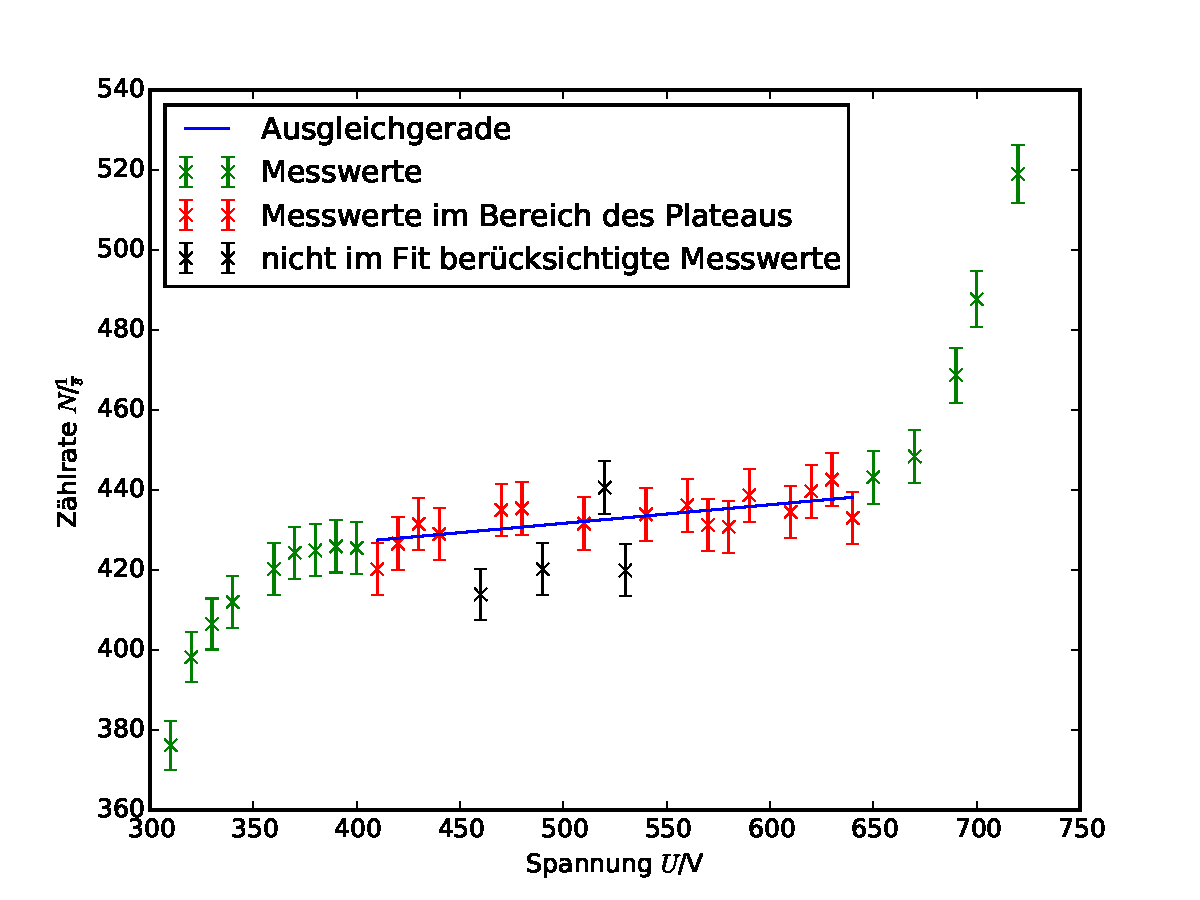
\includegraphics[scale=0.8]{auswertung/plateau.pdf}
\caption{Charakteristik des Zählrohrs mit Ausgleichsgerade im Bereich des Plateaus}
  \label{fig:plateau}
\end{figure}

\begin{table}
  \caption{Zählrate $N$ in Abhängigkeit von der Spannung $U$.}
  \centering
  \label{tab:charakteristik}
  \begin{tabular}{c c}
    \toprule
   $U/\si{\volt}$ & $N /\frac{1}{\si{\second}}$\\
    \midrule
310	& 376,2	\pm 6,13\\
320	& 398,2	\pm 6,31\\
330	& 406,5 \pm 6,38\\
340	& 412,0	\pm 6,42\\
360	& 420,2	\pm 6,48\\
370	& 424,3	\pm 6,51\\
380	& 424,9	\pm 6,52\\
390	& 425,9	\pm 6,53\\
400	& 425,5	\pm 6,52\\
410	& 420,2	\pm 6,48\\
420	& 426,6	\pm 6,53\\
430	& 431,5	\pm 6,57\\
440	& 429,0	\pm 6,55\\
460	& 413,9	\pm 6,43\\
470	& 435,0	\pm 6,60\\
480	& 435,4	\pm 6,60\\
490	& 420,2	\pm 6,48\\
510	& 431,6	\pm 6,60\\
520	& 440,6	\pm 6,64\\
530	& 419,9	\pm 6,48\\
540	& 433,9	\pm 6,59\\
560	& 436,2	\pm 6,60\\
570	& 431,2	\pm 6,57\\
580	& 430,8	\pm 6,56\\
590	& 438,7	\pm 6,62\\
610	& 434,5	\pm 6,59\\
620	& 439,7	\pm 6,63\\
630	& 442,6	\pm 6,65\\
640	& 433,0	\pm 6,58\\
650	& 443,2	\pm 6,66\\
670	& 448,4	\pm 6,70\\
690	& 468,7	\pm 6,85\\
700	& 487,7	\pm 6,98\\
720	& 519,0	\pm 7,20\\
    \bottomrule
    \end{tabular}
\end{table}

Der zeitliche Abstand zwischen Primär- und Nachentladungsimpuls bei geringer Strahlintensität beträgt
\begin{equation}
  \Delta t \approx 225\mu\si{\second}.
\end{equation}

\subsection{Bestimmung der Totzeit}
Zunächst wird die Totzeit $T$ sowie die Erholungszeit $T_\mathrm{E}$ durch Abschätzen auf dem Oszillographen bestimmt.
\begin{align}
  T &= 150 \mu \si{\second}\\
  T_\mathrm{E} &= 300 \mu\si{\second}\\
\end{align}

Außerdem wird die Totzeit mittels der Zwei-Quellen-Methode bestimmt. Für die gemessenen Zählraten lässt sich der Fehler erneut nach Gleichung \ref{eqn:fehler} ermitteln. Somit ergeben sich für die Zählraten folgende Werte:
\begin{align}
  N_1&=(225,890 \pm 4,75) \frac{1}{\si{\second}} \\
  N_2 &= (247,830 \pm 4,98) \frac{1}{\si{\second}} \\
  N_{1+2} &= (377,610 \pm 6,14) \frac{1}{\si{\second}}.
\end{align}
Die Totzeit lässt sich nach
\begin{equation}
  T \approx \frac{N_1+N_2-N_{1+2}}{2N_1N_2}
\end{equation}
berechnen. Da die Werte fehlerbehaftet sind, wird eine Fehlerrechnung mit uncertainties in Python durchgeführt.  Damit ergibt sich:
\begin{equation}
  T\approx (86 \pm 7)\mu\si{\second}.
\end{equation}

\subsection{Freigesetzte Ladungsmenge}
Für die vom Zählrohr freigesetzte Ladung gilt folgender Zusammenhang:
\begin{equation}
  \overline{I} = \frac{\Delta Q}{\Delta t} Z,
\end{equation}
wobei $I$ die gemessenen Stromstärke, $\Delta Q$ der freigesetzten Ladung und $Z$ der Anzahl der Teilchen entspricht, die im Zeitraum $\Delta t$ gemessen werden.
Um den Zusammenhang zwischen der freigesetzten Ladung $\Delta Q$ und der Spannung zu untersuchen, wird $\Delta Q$ aus den gemessenen Stromstärken berechnet und gegen die Spannung $U$ aufgetragen. Dies ist in Abbildung \ref{fig:ladung} dargestellt. Die entsprechnenden Messwerte sowie die freigesetzte Ladung in Einheiten der Elementarladung sind in Tabelle \ref{tab:frei-ladung} zu finden.
Wie Abbildung \ref{fig:ladung} zeigt, ist der Zusammenhang zwischen $\Delta Q$ und $U$ linear. Für die Ausgleichgerade gilt:
\begin{equation}
  \Delta Q = ((3,21 \pm 0.06)\cdot 10^8)\frac{1}{\si{\volt}}x + (893,55 \pm 30,77)\cdot 10^8
\end{equation}

\begin{figure}
  \centering
  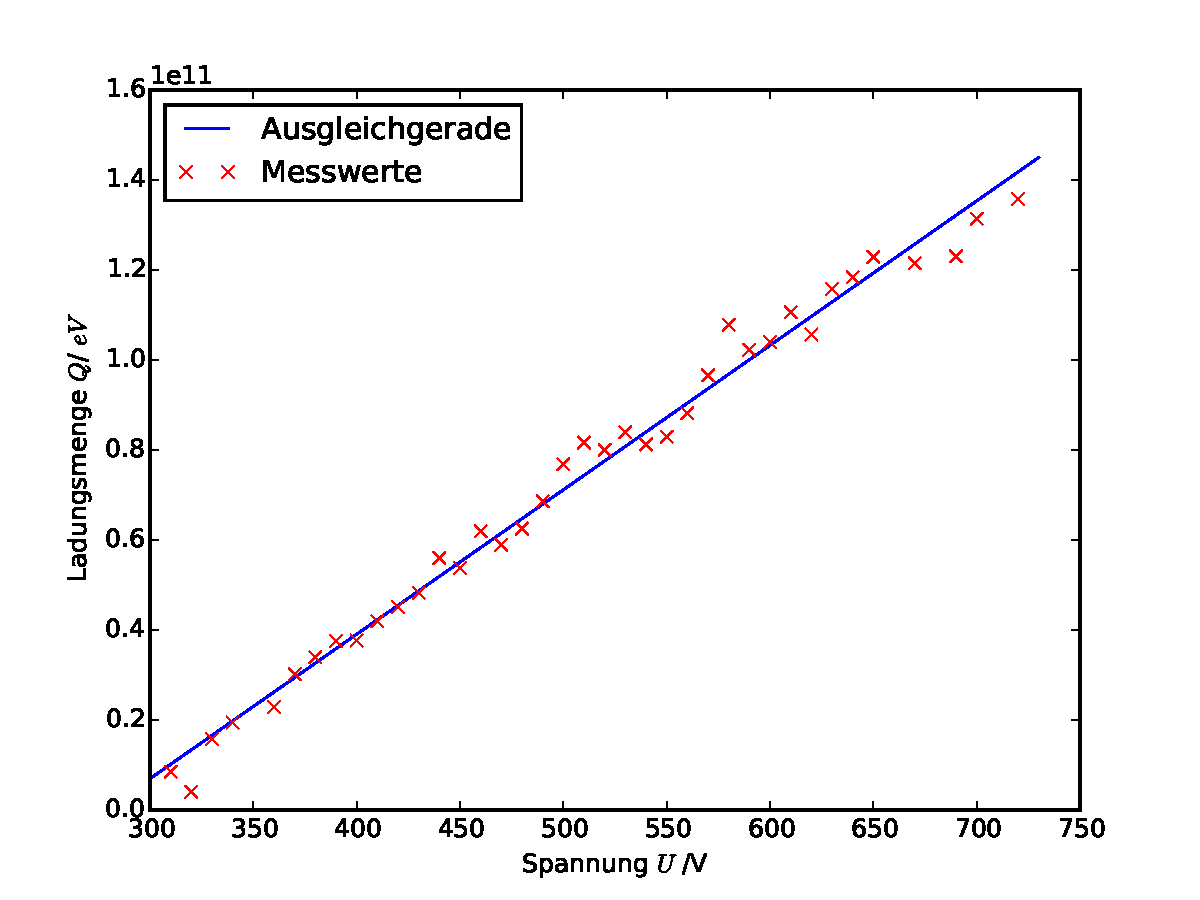
\includegraphics[scale=0.8]{auswertung/d.pdf}
\caption{Freigesetzte Ladung $\Delta Q$ in Abhängigkeit von der Spannung $U$}
  \label{fig:ladung}
\end{figure}

\begin{table}
  \caption{Stromstärke $I$, Impulszahl $n_\mathrm{Impuls}$ und die daraus berechnete freigesetzte Ladungsmenge $\Delta Q$ in Abhängigkeit von der Spannung.}
  \centering
  \label{tab:frei-ladung}
  \begin{tabular}{c c c c c}
    \toprule
   $U/\si{\volt}$ & $I$/$\mu$\si{\ampere} & $n_\mathrm{Impuls}$ & $\Delta Q /\mu \si{\coulomb}$ & $\frac{\Delta Q}{e_0}/10^{10}$\\
    \midrule
320	& 0,1	& 4250 & 0,0002 & 0,12 \\
310	& 0,2	& 3762 & 0,0005 & 0,31\\
330	& 0,4	& 4065 & 0,0010 & 1,58 \\
340	& 0,5	& 4120 & 0,0012 & 1,94 \\
360	& 0,6	& 4202 & 0,0014 & 2,29 \\
370	& 0,8	& 4266 & 0,0019 & 3,00 \\
380	& 0,9	& 4315 & 0,0021 & 3,34 \\
400	& 1,0	& 4312 & 0,0023 & 3,72 \\
390	& 1,0	& 4290 & 0,0023 & 3,73 \\
410	& 1,1	& 4139 & 0,0027 & 4,26 \\
420	& 1,2	& 4350 & 0,0028 & 4,42 \\
430	& 1,3	& 4354 & 0,0030 & 4,78 \\
450	& 1,4	& 4432 & 0,0032 & 5,06 \\
440	& 1,5	& 4202 & 0,0036 & 5,72 \\
470	& 1,6	& 4406 & 0,0036 & 5,81 \\
460	& 1,6	& 4316 & 0,0037 & 5,94 \\
480	& 1,7	& 4199 & 0,0040 & 6,49 \\
500	& 2,0	& 4877 & 0,0041 & 6,57 \\
490	& 1,8	& 4339 & 0,0041 & 6,65 \\
550	& 2,2	& 5190 & 0,0042 & 6,79 \\
540	& 2,2	& 4387 & 0,0050 & 8,03 \\
510	& 2,2	& 4362 & 0,0050 & 8,08 \\
520	& 2,2	& 4312 & 0,0051 & 8,17 \\
530	& 2,2	& 4308 & 0,0051 & 8,18 \\
560	& 2,4	& 4345 & 0,0055 & 8,85 \\
570	& 2,6	& 4397 & 0,0059 & 9,47 \\
620	& 2,9	& 4687 & 0,0062 & 9,91 \\
590	& 2,8	& 4330 & 0,0065 & 10,36 \\
580	& 2,9	& 4426 & 0,0066 & 10,50 \\
600	& 2,8	& 4202 & 0,0067 & 10,68 \\
610	& 3,0	& 4484 & 0,0067 & 10,72 \\
690	& 3,6	& 4687 & 0,0077 & 12,31 \\
640	& 3,2	& 4120 & 0,0078 & 12,44 \\
630	& 3,2	& 4065 & 0,0079 & 12,61 \\
650	& 3,4	& 4243 & 0,0080 & 12,84 \\
670	& 3,4	& 3762 & 0,0090 & 14,48 \\
700	& 4,0	& 4249 & 0,0094 & 15,08 \\
720	& 4,4	& 4259 & 0,010 & 16,55 \\
    \bottomrule
    \end{tabular}
\end{table}
